
%% bare_conf.tex
%% V1.3
%% 2007/01/11
%% by Michael Shell
%% See:
%% http://www.michaelshell.org/
%% for current contact information.
%%
%% This is a skeleton file demonstrating the use of IEEEtran.cls
%% (requires IEEEtran.cls version 1.7 or later) with an IEEE conference paper.
%%
%% Support sites:
%% http://www.michaelshell.org/tex/ieeetran/
%% http://www.ctan.org/tex-archive/macros/latex/contrib/IEEEtran/
%% and
%% http://www.ieee.org/

%%*************************************************************************
%% Legal Notice:
%% This code is offered as-is without any warranty either expressed or
%% implied; without even the implied warranty of MERCHANTABILITY or
%% FITNESS FOR A PARTICULAR PURPOSE! 
%% User assumes all risk.
%% In no event shall IEEE or any contributor to this code be liable for
%% any damages or losses, including, but not limited to, incidental,
%% consequential, or any other damages, resulting from the use or misuse
%% of any information contained here.
%%
%% All comments are the opinions of their respective authors and are not
%% necessarily endorsed by the IEEE.
%%
%% This work is distributed under the LaTeX Project Public License (LPPL)
%% ( http://www.latex-project.org/ ) version 1.3, and may be freely used,
%% distributed and modified. A copy of the LPPL, version 1.3, is included
%% in the base LaTeX documentation of all distributions of LaTeX released
%% 2003/12/01 or later.
%% Retain all contribution notices and credits.
%% ** Modified files should be clearly indicated as such, including  **
%% ** renaming them and changing author support contact information. **
%%
%% File list of work: IEEEtran.cls, IEEEtran_HOWTO.pdf, bare_adv.tex,
%%                    bare_conf.tex, bare_jrnl.tex, bare_jrnl_compsoc.tex
%%*************************************************************************

% *** Authors should verify (and, if needed, correct) their LaTeX system  ***
% *** with the testflow diagnostic prior to trusting their LaTeX platform ***
% *** with production work. IEEE's font choices can trigger bugs that do  ***
% *** not appear when using other class files.                            ***
% The testflow support page is at:
% http://www.michaelshell.org/tex/testflow/



% Note that the a4paper option is mainly intended so that authors in
% countries using A4 can easily print to A4 and see how their papers will
% look in print - the typesetting of the document will not typically be
% affected with changes in paper size (but the bottom and side margins will).
% Use the testflow package mentioned above to verify correct handling of
% both paper sizes by the user's LaTeX system.
%
% Also note that the "draftcls" or "draftclsnofoot", not "draft", option
% should be used if it is desired that the figures are to be displayed in
% draft mode.
%
\documentclass[conference]{IEEEtran}
% Add the compsoc option for Computer Society conferences.
%
% If IEEEtran.cls has not been installed into the LaTeX system files,
% manually specify the path to it like:
% \documentclass[conference]{../sty/IEEEtran}





% Some very useful LaTeX packages include:
% (uncomment the ones you want to load)


% *** MISC UTILITY PACKAGES ***
%
%\usepackage{ifpdf}
% Heiko Oberdiek's ifpdf.sty is very useful if you need conditional
% compilation based on whether the output is pdf or dvi.
% usage:
% \ifpdf
%   % pdf code
% \else
%   % dvi code
% \fi
% The latest version of ifpdf.sty can be obtained from:
% http://www.ctan.org/tex-archive/macros/latex/contrib/oberdiek/
% Also, note that IEEEtran.cls V1.7 and later provides a builtin
% \ifCLASSINFOpdf conditional that works the same way.
% When switching from latex to pdflatex and vice-versa, the compiler may
% have to be run twice to clear warning/error messages.






% *** CITATION PACKAGES ***
%
%\usepackage{cite}
% cite.sty was written by Donald Arseneau
% V1.6 and later of IEEEtran pre-defines the format of the cite.sty package
% \cite{} output to follow that of IEEE. Loading the cite package will
% result in citation numbers being automatically sorted and properly
% "compressed/ranged". e.g., [1], [9], [2], [7], [5], [6] without using
% cite.sty will become [1], [2], [5]--[7], [9] using cite.sty. cite.sty's
% \cite will automatically add leading space, if needed. Use cite.sty's
% noadjust option (cite.sty V3.8 and later) if you want to turn this off.
% cite.sty is already installed on most LaTeX systems. Be sure and use
% version 4.0 (2003-05-27) and later if using hyperref.sty. cite.sty does
% not currently provide for hyperlinked citations.
% The latest version can be obtained at:
% http://www.ctan.org/tex-archive/macros/latex/contrib/cite/
% The documentation is contained in the cite.sty file itself.






% *** GRAPHICS RELATED PACKAGES ***
%
\ifCLASSINFOpdf
  % \usepackage[pdftex]{graphicx}
  % declare the path(s) where your graphic files are
  % \graphicspath{{../pdf/}{../jpeg/}}
  % and their extensions so you won't have to specify these with
  % every instance of \includegraphics
  % \DeclareGraphicsExtensions{.pdf,.jpeg,.png}
\else
  % or other class option (dvipsone, dvipdf, if not using dvips). graphicx
  % will default to the driver specified in the system graphics.cfg if no
  % driver is specified.
  % \usepackage[dvips]{graphicx}
  % declare the path(s) where your graphic files are
  % \graphicspath{{../eps/}}
  % and their extensions so you won't have to specify these with
  % every instance of \includegraphics
  % \DeclareGraphicsExtensions{.eps}
\fi
% graphicx was written by David Carlisle and Sebastian Rahtz. It is
% required if you want graphics, photos, etc. graphicx.sty is already
% installed on most LaTeX systems. The latest version and documentation can
% be obtained at: 
% http://www.ctan.org/tex-archive/macros/latex/required/graphics/
% Another good source of documentation is "Using Imported Graphics in
% LaTeX2e" by Keith Reckdahl which can be found as epslatex.ps or
% epslatex.pdf at: http://www.ctan.org/tex-archive/info/
%
% latex, and pdflatex in dvi mode, support graphics in encapsulated
% postscript (.eps) format. pdflatex in pdf mode supports graphics
% in .pdf, .jpeg, .png and .mps (metapost) formats. Users should ensure
% that all non-photo figures use a vector format (.eps, .pdf, .mps) and
% not a bitmapped formats (.jpeg, .png). IEEE frowns on bitmapped formats
% which can result in "jaggedy"/blurry rendering of lines and letters as
% well as large increases in file sizes.
%
% You can find documentation about the pdfTeX application at:
% http://www.tug.org/applications/pdftex





% *** MATH PACKAGES ***
%
%\usepackage[cmex10]{amsmath}
% A popular package from the American Mathematical Society that provides
% many useful and powerful commands for dealing with mathematics. If using
% it, be sure to load this package with the cmex10 option to ensure that
% only type 1 fonts will utilized at all point sizes. Without this option,
% it is possible that some math symbols, particularly those within
% footnotes, will be rendered in bitmap form which will result in a
% document that can not be IEEE Xplore compliant!
%
% Also, note that the amsmath package sets \interdisplaylinepenalty to 10000
% thus preventing page breaks from occurring within multiline equations. Use:
%\interdisplaylinepenalty=2500
% after loading amsmath to restore such page breaks as IEEEtran.cls normally
% does. amsmath.sty is already installed on most LaTeX systems. The latest
% version and documentation can be obtained at:
% http://www.ctan.org/tex-archive/macros/latex/required/amslatex/math/





% *** SPECIALIZED LIST PACKAGES ***
%
%\usepackage{algorithmic}
% algorithmic.sty was written by Peter Williams and Rogerio Brito.
% This package provides an algorithmic environment fo describing algorithms.
% You can use the algorithmic environment in-text or within a figure
% environment to provide for a floating algorithm. Do NOT use the algorithm
% floating environment provided by algorithm.sty (by the same authors) or
% algorithm2e.sty (by Christophe Fiorio) as IEEE does not use dedicated
% algorithm float types and packages that provide these will not provide
% correct IEEE style captions. The latest version and documentation of
% algorithmic.sty can be obtained at:
% http://www.ctan.org/tex-archive/macros/latex/contrib/algorithms/
% There is also a support site at:
% http://algorithms.berlios.de/index.html
% Also of interest may be the (relatively newer and more customizable)
% algorithmicx.sty package by Szasz Janos:
% http://www.ctan.org/tex-archive/macros/latex/contrib/algorithmicx/




% *** ALIGNMENT PACKAGES ***
%
%\usepackage{array}
% Frank Mittelbach's and David Carlisle's array.sty patches and improves
% the standard LaTeX2e array and tabular environments to provide better
% appearance and additional user controls. As the default LaTeX2e table
% generation code is lacking to the point of almost being broken with
% respect to the quality of the end results, all users are strongly
% advised to use an enhanced (at the very least that provided by array.sty)
% set of table tools. array.sty is already installed on most systems. The
% latest version and documentation can be obtained at:
% http://www.ctan.org/tex-archive/macros/latex/required/tools/


%\usepackage{mdwmath}
%\usepackage{mdwtab}
% Also highly recommended is Mark Wooding's extremely powerful MDW tools,
% especially mdwmath.sty and mdwtab.sty which are used to format equations
% and tables, respectively. The MDWtools set is already installed on most
% LaTeX systems. The lastest version and documentation is available at:
% http://www.ctan.org/tex-archive/macros/latex/contrib/mdwtools/


% IEEEtran contains the IEEEeqnarray family of commands that can be used to
% generate multiline equations as well as matrices, tables, etc., of high
% quality.


%\usepackage{eqparbox}
% Also of notable interest is Scott Pakin's eqparbox package for creating
% (automatically sized) equal width boxes - aka "natural width parboxes".
% Available at:
% http://www.ctan.org/tex-archive/macros/latex/contrib/eqparbox/





% *** SUBFIGURE PACKAGES ***
%\usepackage[tight,footnotesize]{subfigure}
% subfigure.sty was written by Steven Douglas Cochran. This package makes it
% easy to put subfigures in your figures. e.g., "Figure 1a and 1b". For IEEE
% work, it is a good idea to load it with the tight package option to reduce
% the amount of white space around the subfigures. subfigure.sty is already
% installed on most LaTeX systems. The latest version and documentation can
% be obtained at:
% http://www.ctan.org/tex-archive/obsolete/macros/latex/contrib/subfigure/
% subfigure.sty has been superceeded by subfig.sty.



%\usepackage[caption=false]{caption}
%\usepackage[font=footnotesize]{subfig}
% subfig.sty, also written by Steven Douglas Cochran, is the modern
% replacement for subfigure.sty. However, subfig.sty requires and
% automatically loads Axel Sommerfeldt's caption.sty which will override
% IEEEtran.cls handling of captions and this will result in nonIEEE style
% figure/table captions. To prevent this problem, be sure and preload
% caption.sty with its "caption=false" package option. This is will preserve
% IEEEtran.cls handing of captions. Version 1.3 (2005/06/28) and later 
% (recommended due to many improvements over 1.2) of subfig.sty supports
% the caption=false option directly:
%\usepackage[caption=false,font=footnotesize]{subfig}
%
% The latest version and documentation can be obtained at:
% http://www.ctan.org/tex-archive/macros/latex/contrib/subfig/
% The latest version and documentation of caption.sty can be obtained at:
% http://www.ctan.org/tex-archive/macros/latex/contrib/caption/




% *** FLOAT PACKAGES ***
%
%\usepackage{fixltx2e}
% fixltx2e, the successor to the earlier fix2col.sty, was written by
% Frank Mittelbach and David Carlisle. This package corrects a few problems
% in the LaTeX2e kernel, the most notable of which is that in current
% LaTeX2e releases, the ordering of single and double column floats is not
% guaranteed to be preserved. Thus, an unpatched LaTeX2e can allow a
% single column figure to be placed prior to an earlier double column
% figure. The latest version and documentation can be found at:
% http://www.ctan.org/tex-archive/macros/latex/base/



%\usepackage{stfloats}
% stfloats.sty was written by Sigitas Tolusis. This package gives LaTeX2e
% the ability to do double column floats at the bottom of the page as well
% as the top. (e.g., "\begin{figure*}[!b]" is not normally possible in
% LaTeX2e). It also provides a command:
%\fnbelowfloat
% to enable the placement of footnotes below bottom floats (the standard
% LaTeX2e kernel puts them above bottom floats). This is an invasive package
% which rewrites many portions of the LaTeX2e float routines. It may not work
% with other packages that modify the LaTeX2e float routines. The latest
% version and documentation can be obtained at:
% http://www.ctan.org/tex-archive/macros/latex/contrib/sttools/
% Documentation is contained in the stfloats.sty comments as well as in the
% presfull.pdf file. Do not use the stfloats baselinefloat ability as IEEE
% does not allow \baselineskip to stretch. Authors submitting work to the
% IEEE should note that IEEE rarely uses double column equations and
% that authors should try to avoid such use. Do not be tempted to use the
% cuted.sty or midfloat.sty packages (also by Sigitas Tolusis) as IEEE does
% not format its papers in such ways.





% *** PDF, URL AND HYPERLINK PACKAGES ***
%
%\usepackage{url}
% url.sty was written by Donald Arseneau. It provides better support for
% handling and breaking URLs. url.sty is already installed on most LaTeX
% systems. The latest version can be obtained at:
% http://www.ctan.org/tex-archive/macros/latex/contrib/misc/
% Read the url.sty source comments for usage information. Basically,
% \url{my_url_here}.





% *** Do not adjust lengths that control margins, column widths, etc. ***
% *** Do not use packages that alter fonts (such as pslatex).         ***
% There should be no need to do such things with IEEEtran.cls V1.6 and later.
% (Unless specifically asked to do so by the journal or conference you plan
% to submit to, of course. )


% correct bad hyphenation here
\hyphenation{op-tical net-works semi-conduc-tor}


\begin{document}
%
% paper title
% can use linebreaks \\ within to get better formatting as desired
\title{On the self adaptiveness in \\Wireless Sensor Networks}


% author names and affiliations
% use a multiple column layout for up to three different
% affiliations
\author{
\IEEEauthorblockN{Mikhail Afanasov}
\IEEEauthorblockA{Politecnico di Milano\\
afanasov@elet.polimi.it}
\and
\IEEEauthorblockN{Sonda Bousnina}
\IEEEauthorblockA{Politecnico di Milano\\
sonda.bousnina@ieee.org}
\and
\IEEEauthorblockN{Giuseppe Massari}
\IEEEauthorblockA{Politecnico di Milano\\
giuseppe.massari@polimi.it}
\and
\IEEEauthorblockN{Vincenzo Sciancalepore}
\IEEEauthorblockA{Politecnico di Milano\\
vincenzo.sciancalepore@imdea.org}
}

% conference papers do not typically use \thanks and this command
% is locked out in conference mode. If really needed, such as for
% the acknowledgment of grants, issue a \IEEEoverridecommandlockouts
% after \documentclass

% for over three affiliations, or if they all won't fit within the width
% of the page, use this alternative format:
% 
%\author{\IEEEauthorblockN{Michael Shell\IEEEauthorrefmark{1},
%Homer Simpson\IEEEauthorrefmark{2},
%James Kirk\IEEEauthorrefmark{3}, 
%Montgomery Scott\IEEEauthorrefmark{3} and
%Eldon Tyrell\IEEEauthorrefmark{4}}
%\IEEEauthorblockA{\IEEEauthorrefmark{1}School of Electrical and Computer Engineering\\
%Georgia Institute of Technology,
%Atlanta, Georgia 30332--0250\\ Email: see http://www.michaelshell.org/contact.html}
%\IEEEauthorblockA{\IEEEauthorrefmark{2}Twentieth Century Fox, Springfield, USA\\
%Email: homer@thesimpsons.com}
%\IEEEauthorblockA{\IEEEauthorrefmark{3}Starfleet Academy, San Francisco, California 96678-2391\\
%Telephone: (800) 555--1212, Fax: (888) 555--1212}
%\IEEEauthorblockA{\IEEEauthorrefmark{4}Tyrell Inc., 123 Replicant Street, Los Angeles, California 90210--4321}}




% use for special paper notices
%\IEEEspecialpapernotice{(Invited Paper)}




% make the title area
\maketitle


\begin{abstract}
This work aims at providing a report, showing some noticeable example of
self-configuration (or self-adaptation) approaches in the context of Wireless
Sensor Networks (WSNs). Although this cannot be considered an exhaustive survey,
we are confident about the fact that this work includes enough information to
motivate and justify the exploitation of self-adaptiveness techniques in the design
of such systems.

\end{abstract}

\IEEEpeerreviewmaketitle

% Section I
\section{Introduction}
\label{sec:in}
Wireless Sensor Network (WSN) is a set of tiny distributed wireless nodes that have to collaborate and cooperate on a common distributed application to perform tasks specified by a user (Fig.~\ref{fig:scenario}). Recently, the development of WSNs has received an increasing interest due to the fast technological advances in the fields of sensor technology, low power microelectronics, and low energy wireless communications.
These networks are currently used in wide range of applications in the scientific, medical, commercial, and military domains, like for instance home automation, environment monitoring, industrial control, surveillance, security, healthcare, etc. 

In this context, WSNs are intimately tied to and inherently dependent on an environment they operate in. It leads to a necessity to adapt to an unpredicted environmental dynamics. Adaptation at run-time provides more flexibility in such software behavior as energy management, network protocols, architecture reconfiguration and error handling.
In fact, the application of self-organization concept to wireless sensor networks is seen as a key driver for improving the operation and maintenance of these networks. Thus, the self-organization can help reducing the cost of installation and management by simplifying some operational tasks through automated mechanisms pointing the self-configuration, self-optimization and self-healing~\cite{son_marchetti}.
Regarding self-configuration, it is triggered by incidental events for instance to add a new site or to introduce a new service or a new network feature. In that case, these lasts can require a re-configuration of a number of radio parameters or several resource management algorithms.
For the self-optimization in WSNs, intelligent methods are applied to the processed measurements to derive an updated set of the radio parameters or the resource management parameters~\cite{son_marchetti}.
Sensor nodes and wireless links are subject to different errors in function of the size of perturbation in time, space, and energy. So applying self-healing methods can resolve these problems and the loss of coverage or capacity induced by such events~\cite{son_marchetti}.
In this regard, WSNs increasingly need self-organization, self-configuration and self-adaptation to changing conditions to ease management and operation~\cite{son_sengul}.


\begin{figure}[t]
\vspace{-4mm}
\centering
 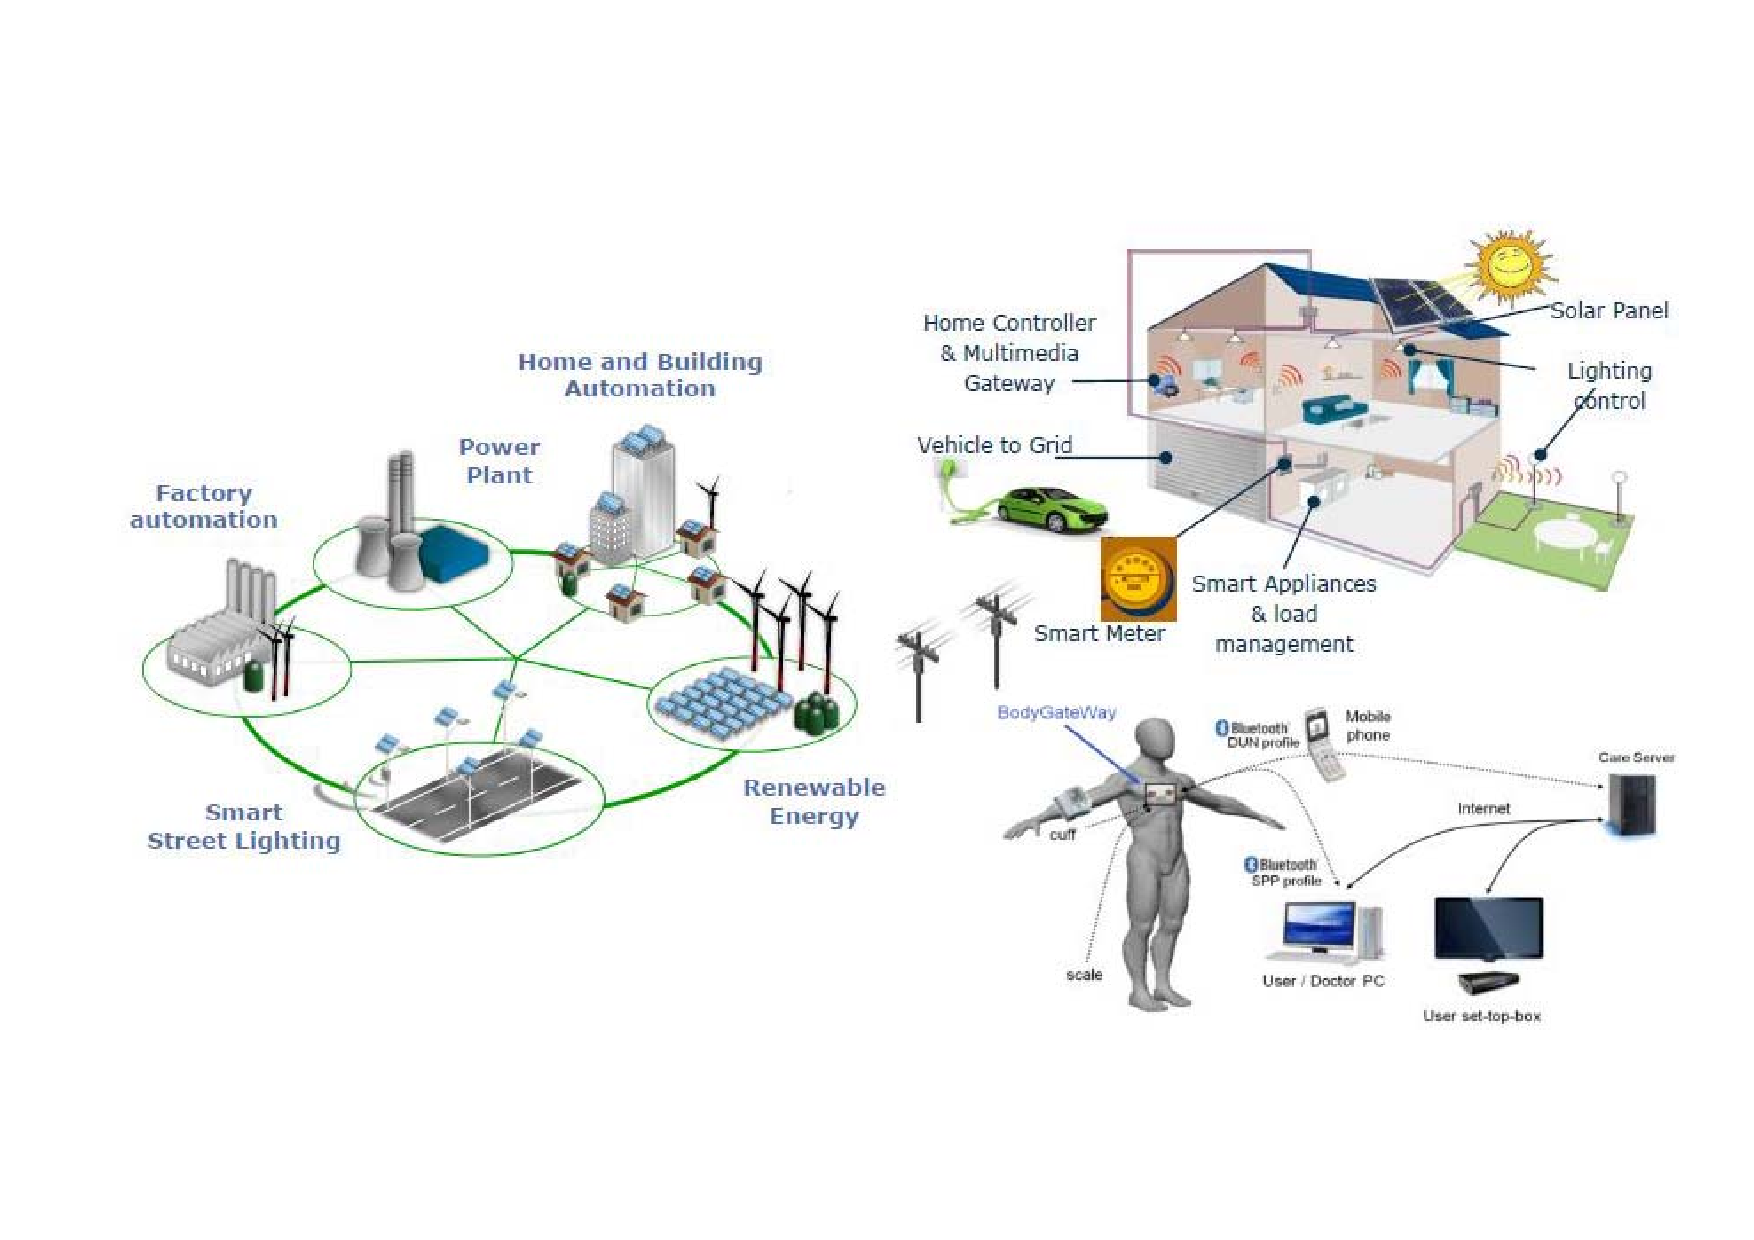
\includegraphics[width=\columnwidth]{fig/fig}
 \vspace{-4mm} 
 \caption{Examples of wireless sensor networks.}
 \vspace{-4mm}
  \label{fig:scenario}
\end{figure}


In this respect, fits the present work.
The remainder of this report is organized as follows. In section
\ref{sec:sa}, we present some related works in a sort of a state of the art
about self configuration of WSNs. This section is subdivided in three parts
describing respectively the concept of self configuration related to the WSNs architecture, the applications and services in these networks, and the systems
and networking in these lasts. Overall evaluations about the works are
discussed in Section~\ref{sec:ev}. Finally, Section~\ref{sec:conclusions} concludes the paper.


% Section II
\section{State of the Art}
\label{sec:sa}
In this section we group a set of relevant works focusing on the exploitation of
self-adaptive and self-configuring approaches in WSN. We identified three
perspectives, according to the targeted objective they face with. The
\emph{architecture} perspective looks at the WSN from the point of view of the
topology, by adapting it to network dynamics, i.e. link failures, sensor nodes
discovering and region covering.
The \emph{application} perspective copes with problems related to programming
models, i.e. to deploy the application on a distributed system, update it, adapt
the behavior of the software to changing environments.
The \emph{system} perspective aims at optimizing the resource usage, since WSN
are very resource-constrained. We can perform energy management, taking into
account QoS, by adapting network protocols, transmission power and duty-cycle
efficiency enhancement.





\subsection{Architecture}
\label{ssec:sa_app}
There is a significant part of work devoted to a self-addictiveness on an
architectural level~\cite{}. Research in this area is focused mainly on such
properties of the network as: topology, positioning of nodes, fault-tolerance
and scalability. Unlike the other levels, architectural level implies a set of
communicating and collaborating nodes.

\subsubsection*{An architecture for building self-configurable systems}

Subramanian et al.~\cite{subramanian00} focused on the self-organizing architecture for WSNs and
proposed components necessary for building such an architecture. The latter
implies following components:

\begin{itemize}
\item \emph{Specialized sensors} for monitoring different physical entities.
\item \emph{Routing sensors} provide a data dissipation and fault tolerance of the network.
\item \emph{Aggregator nodes} combine routing and sensor functionality to
provide a better network flexibility.
\item \emph{Sink nodes} have a high storage capacity, store and process received data.
\end{itemize}
All the components mentioned above are sufficient for building a wide range of
applications, where infrastructure consists of addressing, routing, broadcasting
and multicasting mechanisms.

Given the proposed architectural components, author also propose four steps,
which should be performed by the network to self-organize:

\begin{itemize}
\item \emph{Discovery phase.} Each node discovers its neighbors.
\item \emph{Organizational phase.} Nodes are organizing groups, allocate
addresses, build routing table and construct broadcast tree and graph spanning
all nodes.
\item \emph{Maintenance phase.} Each node keeps track of its energy, constantly
updates routing table, broadcast trees and graphs, sends \emph{I am alive}
message and routing table to its neighbors.
\item \emph{Self-Reorganization phase.} If node detects the failure of its
neighbor, it updates its routing table, or starts \emph{Discovery phase} in case
of the failure of all of the neighbors.
\end{itemize}

The analysis of the approach shows that the hierarchy of the network is strictly
balanced; the complexity of the routing is \emph{O(}log~\emph{n)}; the network is
extremely tolerant to either node or link failures; the uniqueness property is
guaranteed by the presence of a hierarchy; specialized sensors are allowed to be
mobile. There are several weaknesses of the approach, though. Thereby,
the approach is not optimized for extremely dynamic systems, when the network
changes badly or very fast. On the other hand, the required protocol for such
networks is not discussed. Despite the specialized sensors can be mobile, they
can not move beyond the reach of routers. The latter, however are considered static.

The approach is very well fitted for static WSN, such as one for collecting
meteorological data. But it is absolutely not applicable for systems with high
dynamics such as wildlife monitoring~\cite{Pasztor10}, since the network changes
badly and rapidly.


\subsection*{ASCENT: Adaptive Self-Configuring Sensor Networks Topologies}
In \cite{ascent} the authors provide an other self-configuring approach in order to deploy micro-sensor for a wide range of environmental monitoring applications. They assumed a very-dense scenario where is extremely necessary to find a trade-off between the sensors' coverage and the interferences due to the large number of involved sensors. The real scenario given by that work is a habitat monitoring sensor network that is deployed in a remote forest, where the sensors are dropped by a plane.
Different aspects are taken into account and then analysed: power consumption as well as the distributed sensing task. The work seems to be very interesting for two different reasons: first, adaptive techniques implied permit applications to configure the underlying topology based on their needs by trying to save energy and extend the network lifetime, second, the self-adaptive approach is based on the operating conditions measured locally.
Specifically, the authors identify two kinds of sensors, namely nodes, in the network: \textit{i) active} and \textit{ii)} passive. The active nodes stay awake all the time and perform routing procedure, while the passive nodes listen the channel and periodically check if they should turn into active mode. The active nodes will be in charge of producing messages (sources) or just disseminating them (sink). In the case of low channel condition, the sink nodes could send an \textit{help message} to other passive node in order to activate them.
The self-configuring process starts by turning on randomly some nodes in the network. Such nodes enter firstly in a test mode, where they can exchange data and routing control messages, so that after a prefixed time can be switched to an active mode. If there are too many neighbour nodes active, according to a fixed parameter, the node will be switched off. Afterwards, if the number of active neighbour nodes will be less than a prefixed parameter and the data loss rate good enough it will be re-activated. 
Note that the performance of the system depend on the parameters chosen. The work provide a good validation for the parameters provided by analysing and comparing the network performance in terms of energy savings and network capacity. The gain of power saving is a factor of $3$ better in some dense cases.

\subsection{Application}
\label{ssec:sa_app}

From an application perspective the challenges introduced by WSN are basically
related to their distributed architecture, the scarceness of resources of the single
sensor node, and the reliability issues due to sensor nodes disappearing for
unpredictable faults, communication noises or battery discharging.
\\
This requires the development of ad-hoc programming models that could fit in the
architectural view of the WSN, and that allow the application to react and adapt
to environmental changes.
This section introduces some approaches addressing this kind of problem.

\subsection{COPAL-ML: A Macro Language for Rapid Development of Context-Aware
Applications in Wireless Sensor Networks}

Sehic et. al~\cite{sehic11} propose a Java based API for developing self-adaptive
applications for WSNs. By using this framework developer can specify the way the
contextual data will be collected, processed and used by the application.
COPAL-ML implies such components as:

\begin{itemize}
\item \emph{Context type} specifies the format of the data provided by a WSN.
\item \emph{Publisher} periodically publishes an information about a specific
context type.
\item \emph{Listener} handles an event fired by the publisher and receives a
context type as an argument.
\item \emph{Processor} handles the received data.
\end{itemize}

Along with possible scenario, authors also proposed several processing patterns,
which can be used as solutions for effective self-adaptive application. Despite it
is very promising way towards abstraction of WSN on the high level, the
framework is Java-based, thus, it is applicable for very limited range of sensor
nodes. It is possible, however, to run the framework on the machine with an
unlimited energy source, but in this case the communication between the
framework and the node remains unclear.

\subsubsection*{Supporting Lightweight Adaptations in Context-aware
Wireless Sensor Networks}

A common problem with WSN is to deploy an application, or update it, when the
sensor network features a lot of nodes spread over a wide or region. As well,
reprogramming a whole WSN deployed in a inaccessible region, represents a
cumbersome, and often unfeasible, activity. Thus, the challenge is to support
these operations in a feasible way, at the price of the lowest possible
overhead.
\\
Apart from this issues, a typical requirement of applications like
\emph{environmental monitoring} is to adapt the behavior of the nodes to the
dynamics introduced by events, as for instance the presence or people moving
around or not. 
\\
The work of Taherkordi et \emph{al.}\cite{app:taherkordi}, introduces the
\texttt{WiSeKit} distributed middleware, along with the \texttt{ReWiSe} software
component model, as a solution to support a lightweight behavioral adaptation of
sensor networks. The \texttt{WiSeKit} middleware exposes the following services
\begin{itemize}
	\item \emph{Local Reasoning} to update the values of components’ parameters
		based on a local adaptation policy.
	\item \emph{Adaptation Proxy} to receive adaptation request from cluster
		head.
	\item \emph{Component Repository} to temporarily store a new component’s
		image.
	\item \emph{Component Reconfigurator} to load, reload or remove a running
		component.
\end{itemize}
The \texttt{ReWiSe} component model considers the application as an integration
of separate components. A component can be dynamically replaced, Reconfiguration
in  WSN can be a very expensive operation, since it requires to transfer code to
sensor nodes, to save and resume of state information, and eventually restart
the sensor node. The main costs are paid in terms of \emph{energy consumption}
and are proportional to the size of the code images to transfer. For this
reason, the goal of this work has been to develop a software component model
that i) enables the possibility of a fine-grained reconfiguration of the
application, ii) reduce the overhead due to state saving.
The framework has been implemented on top of the \texttt{Contiki} operating
system. Preliminary experiments reported a decrease of energy consumption of
about $75\%$, compared to a common software component model.




\subsection{System}
\label{ssec:sa_sys}
The system level requires a lot of coordination between distinct sensors in the
network. Particularly, several works leverage the WSN capabilities in order to
reduce power consumption, make the MAC layer more flexible, and perform routing
in a very efficient way. We take into consideration some of them in order to
cover the main categories of system level improvements in the WSN.
\subsubsection{Proactive Reconfiguration of Wireless Sensor Networks}
\label {ssec:proactive}

Steine at \emph{al.} in \cite{sys:proactive} leverage on the exploitation of a
design-time exploration, to identify a set of operating modes. At run-time the
WSN can adapt its behavior to environmental conditions and QoS fluctuations,
by reconfiguring itself into the most suitable operating mode.  The paper
defines an \emph{operating mode} as a set of values assigned to some
controllable parameters of the network protocols.
The nodes can dynamically change, at run-time, their operating mode according to
specific observable events, that potentially affect the QoS of the WSN. The
events are detected using sensors and/or the current time of the day. This
figures out a \emph{proactive} approach in the self-adaptive behavior.
Concerning the network parameters, it is worth to distinguish between
\emph{local} and \emph{global} parameters. In the former case, the single node
can independently reconfigure itself without affecting the others. For instance,
the tuning of the transmission power. In the latter, changing a global parameter
necessarily requires a synchronization step, in order to maintain the proper
functioning of the WSN. Example of global parameters are the TDMA slot-size and
the sleep-time of the nodes.
Thus, whenever a node detect an event, it can immediately adapt its local
parameters or notify the other nodes about the need of change the current global
mode.
The authors have demonstrated the validity of the approach by testing it in a
"cow-health" and a "office" monitoring scenarios. The evaluation metrics
considered are the average delivery ratio and the average power consumption. In
both the scenarios it has been experienced a significant reduction of power
consumption, comparing the approach to a single configuration (worst-case) not
adaptive design. This, keeping the packets delivery ratio close the values
related to the worst-case based design.


\subsection{pTunes: Runtime Parameter Adaptation for Low-power MAC Protocols}

The work of Zimmerling et al. is focused on an adaptation of system level -- MAC protocol. The proposed framework -- pTunes -- allows to adjust the parameters of protocols to adapt to link, topology, and traffic dynamics. To this end, authors analyze the vital parameters -- both protocol dependent and protocol independent -- of the network, such as: reliability, latency and life-time. The framework also meets such requirements as: minimum disruption, timeliness, consistency and energy efficiency.

Evaluation section of the work shows that the framework enhance the network lifetime, effectively controls the traffic and keeps the QoS even when link quality is very low. The approach, however, is centralized, thus it is impossible to perform per-node adjustment. It is also unclear, how much protocols are supported by the framework.
\subsection*{Reducing Energy Consumption}
From an energy saving perspective, interesting approaches have been proposed in the literature. One of them just exploits the idea that the energy used for communication in a sensor network can me improved by decreasing the communication range. The transmission energy is proportional to the distance between the transmitters. Therefore, in \cite{??} they propose a self-adaptive methodology which reduce in an optimal fashion the distances between the main nodes in the network (BS) and the other sensors communicating with it as well as optimizes the number of active sensors by keeping the redundancy at good levels. 
The authors just divide the approach in two phases: the former is to identify the right location for the main sensor, which aims at minimizing the distances with the other sensor nodes, the latter is to switch off the nodes which are useless for covering the area. Additionally, since the nodes communicate by broadcasting messages, they suggested a smart solution which just enables in turn the active node to sense the channel in order to cope with the collision problem. The results are pretty good in terms of power saving. Interestingly, the proposed method not only reduces overall energy consumption of the network but also the lifetime of the nodes is increased significantly.




% Section III
\section{Evaluations}
\label{sec:ev}
compare different approaches to self-adaptive (self-configurable) WSNs

\bibliographystyle{IEEEtran}
\bibliography{report}


\end{document}
